\documentclass{article}
\usepackage[utf8]{inputenc}

\usepackage{siunitx} % \SI{50}{\nano\second}
\usepackage{booktabs}
\usepackage{tabularx}
\usepackage{amsmath}
\usepackage{amssymb}
\usepackage{amsfonts}
\usepackage{graphicx}
\usepackage{float}
\usepackage{caption}
\usepackage{subcaption}
\usepackage{bm} % e.g., \bm(\mu)
\usepackage{xfrac}  % e.g., \sfrac{1}{2}                   
\usepackage{relsize} % e.g., \mathlarger 
\usepackage{algorithm2e}
\DeclareMathOperator*{\argmax}{arg\,max}
\DeclareMathOperator*{\argmin}{arg\,min}

\usepackage[sorting=none,citestyle=numeric-comp, bibstyle=ieee, dashed=false]{biblatex}
\usepackage[colorlinks=true,
		     allcolors=black]{hyperref}
\addbibresource{bibliography.bib}



\title{MSM Hyperparameter Optimisation}
\author{Robert Arbon, Antonia Mey}
\date{November 2020}

\begin{document}

\maketitle

% Introduction/Synopsis:
% MSMs have hyperparameters which affect model predictions/observables 
% Choosing best hyperparameters difficult because dimensionality. 
% Problem tackled in machine learning literature using BO and RSs. 
% Random sampling better than grid because some HPs have high relevance. 
% BO good when MSM evaluations are expensive and HP high relevance. 
% Current practice is a bit ad-hoc. 

% Method: 
% Decision tree:
% You know little about the model
% Random sampling
% Fit RS
% Check for convergence. 
% Use BO if convergence is slow (time)
% You know that some parameters have high relevance
% Use BO
% All parameters have low relevance
% Use Random Sampling


Fundamentally this paper is a bit weak and I've been trying multiple introductions to try and shape it into something interesting and future proof without actually doing the calculations. I'm going to abandon this approach now, as I've been going round in circles. 

Questions/comments for Toni: 

1. There is a multiplicative explosion of Protein/feature combinations. I suggest we pick one or two proteins and some features which are a bit different.  The WW-domain has been studied the most with the widest variety of features. See heat map of protein/feature combinations  below. Let me know what you think. 
2. Unlike my thesis, I'm not considering protein features a hyperparameter to be modelled with response surfaces and optimised with Bayesian optimisation.  So a response surface will be for all the other hyperparameters.  e.g., the for WW-domain with backbone dihedrals, there will be a response surface with number of cluster centers, TICA params etc. 
3. Please read the intro and the results/discussion sections for general shape of paper.  The methods section is there if you want details.  
4. I've added the bit in about spectral gaps as Tiwary recently released a paper about its importance for ML models.  It's my proxy for a CK test as it's a nice continuous variable and is actually related to the fundamental approximation for MSMs. ]
5. There's a lot that can be cut. 



\begin{figure}
    \centering
    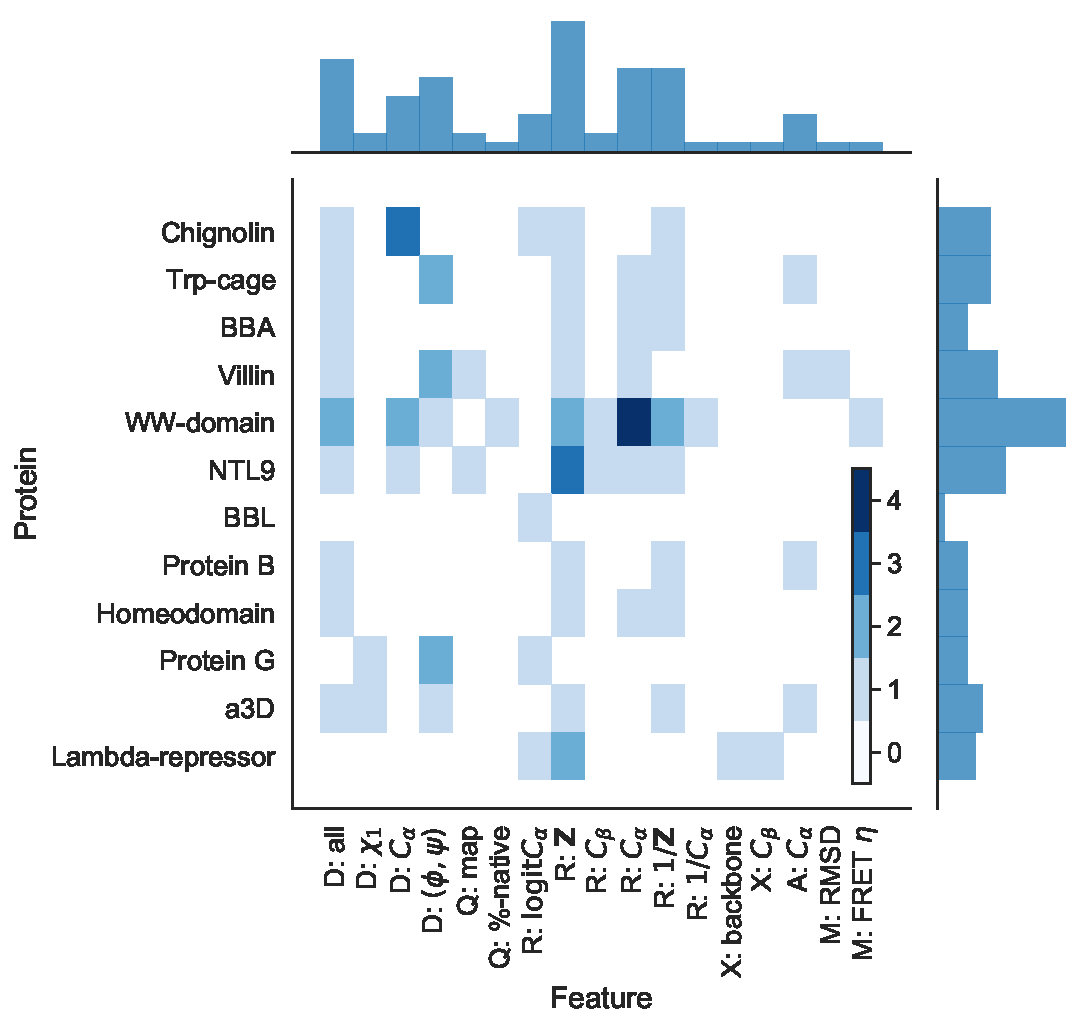
\includegraphics[width=0.9\textwidth]{figures/background_features.pdf}
    \caption{Proteins studied (vertical) and features selected (horizontal) in every paper using the desres data with MSMs.  D = dihedrals, Q = contacts, R = inter-residue distances, X = positions, A = proper angles.  Z = heavy atoms.  so the most popular feature is the inter residue  distances measured on heavy atoms. The most common protein/feature combination is WW-domain with inter residue distance measured on alpha carbons (4 papers). }
    \label{fig:my_label}
\end{figure}


\section{Introduction}

Markov state models (MSM) continue to be a popular tool for determining collective variables, kinetic and thermodynamics of complex dynamical systems. Starting with a set of molecular dynamic (MD) simulations, a series of processing steps is performed to create trajectories of discrete states. Using these, the probabilities of state-to-state transitions, separated by a time $\tau$, are estimated giving a discrete approximation to the system's Markov operator. Finally, its eigenvectors and eigenvalues, which represent the relaxation processes and their timescales, are used to extract all relevant kinetic and thermodynamic information. In particular the $k$ slow relaxation processes, separated from the fast relaxation processes by a significant gap in their implied timescales, define the metastable states and contribute most to observables of interest. The accuracy of the model is then strongly influenced by how well the discrete basis states are able to capture these slow eigenvectors. The processing steps, or hyperparameters, which determine the discrete states must therefore be chosen with care. 

Over the past decade  a firm theoretical foundation for estimating and tuning MSM hyperparameters has been established. The variational approach to conformational dynamics (VAC) established choosing  basis states able to capture the slow Markov eigenvectors as an variational optimisation problem. The generalized matrix Rayleigh coefficient (GMRQ) was introduced which allowed the scoring of hyperparameter choices while avoiding over-fitting with cross-validation. The variational approach to Markov processes (VAMP) generalized VAC to encompass nonreversible dynamics and extended the number of scoring functions. 

These theoretical developments helped establish the following MSM construction pipeline:  first, an appropriate feature ($\chi$) of the system is chosen which  captures its slow dynamics. For example, the flexible backbone torsion angles of a peptide for protein folding. After `featurizing' the trajectories, a small number ($m$) of linear combinations of these features which approximates the slow dynamics are estimated using  time-independent component analysis (TICA) with a given lag time ($\tau_{\mathrm{TICA}}$). Clustering using e.g., k-means, is used to create $n$ discrete Markov states and estimate the Markov state model. The VAMP score of the MSM can then be used to judge the values of $\chi, m, \tau_{\mathrm{TICA}}$ and $n$ (collectively $\mathbf{x}$). The process of choosing $\mathbf{x}$, fitting an MSM and evaluating using VAMP scores can be repeated until satisfactory convergence of VAMP scores, a process known as hyperparameter tuning. 

Husic et. al. were among the first to explicitly apply hyperparameter tuning to the problem of MSMs by randomly sampling hyperparameters and selecting the model with the highest cross-validated GMRQ. Scherer et. al. developed a multifidelity tuning approach, by first scoring the featurized trajectories using an approximate VAMP score without estimating a full MSM. This allows selection of a protein feature before going on to tune other hyperparameters. While these approaches were important steps towards a truly reproducible and transparent method for estimating MSMs, several practical questions remain unanswered. First, at what point is convergence in the VAMP scores reached? Second, how can one efficiently reach the optimum values of VAMP scores and hyperparameters? 

The machine learning community have been active in answering these questions where large machine learning models can take hour or days to train, precluding the ability to exhaustively search the space of potential hyperparameter combinations.  Bayesian optimisation has proven itself a powerful technique for optimising functions, $f(\cdot)$, which are expensive to evaluate with no gradient information (so called ``black-box`` functions). The core of the BO method for hyperparameter optimisation is to model the response of a model (e.g., the VAMP scores of an MSM) to its hyperparameters (e.g., $\mathbf{x}$) with a statistical regression model: $\hat{f}(\mathbf{x})$. At each stage, $i$,  of the optimisation processes, a value of the hyperparameter vector $\mathbf{x}^{i}$ is chosen which is expected to optimise $\hat{f}_{i-1}(\mathbf{x})$. $\mathbf{x}^{i}$ is then evaluated by the model i.e., $f(\theta^{i})$ and this result used to reestimate the response function $\hat{f}_{i}(\mathbf{x})$.  this process continues until the optimum of $\hat{f}$ reaches some convergence criteria. As noted in [firstorder paper] however, Bayesian optimisation is not always guaranteed to be more efficient than randomly sampling hyperparameters, as in [husic].  Thus the first aim of this paper is to both demonstrate how to use BO to optimise MSMs and when it is necessary.  

However, the VAMP scores themselves are not the objects of interest when creating an MSM.  Typically one is interested in determining metastable states, reactive pathways and their implied timescales.  Nor are VAMP scores the only measure of model quality, importantly they do not address the fundamental assumption for accurate dimensionality reduction - namely a strong separation or gap in the eigenvalue spectrum or implied timescales [tiwary refs, sgoop etc.].  Indeed, the number of dominant eigenvectors which are evaluated in the VAMP score is itself  hyperparameter of the modelling process - but one for which there is no optimisation principal to guide its selection.  It is possible then to optimise a VAMP score but miss important slow processes by selecting too few eigenvectors; or to choose hyperparameters which optimise many fast processes at the expense of the dominant eigenvectors, by choosing too many eigenvectors. 
In addition, it is not clear how MSM hyperparameters affect the eigenvalue separation and thus the validity of the model.  

The second aim of this paper is to determine how optimising VAMP scores, in particular in the case where the VAMP score itself is mis-specified, affects the fundamental assumption of a spectral gap. To do this, we extend the response surface modelling used for Bayesian optimisation to describe the sensitivity of the spectral gap to hyperparameters and the VAMP score. 


Question 1: Do different feature correspond to different models? 
Question 2: Does different VAMP scores correspond to different models? 
Question 3: For a given feature, do other hyperparameters matter? 
Question 4: How sensitive are model observables and VAMP scores to hps? 

Q1 and 2 answered by compare-path-chart.ipynb

\section{Theory}
\subsection{MSMs}
To construct a Markov state model one first pre-processes a set of molecular dynamics trajectories into trajectories of discrete states which approximate a Markov chain. Transitions between states separated by a time $\tau$ are counted and used to estimate the Markov transition matrix through either maximum likelihood or Bayesian estimation.

Finish. 

\subsection{Gaussian Processes}

copy from thesis
% A Gaussian process is a distribution over functions \cite{rasmussenGaussianProcessesMachine2006}.  In other words, drawing a sample from a GP gives a continuous function $f(\mathbf{x})$, where $\mathbf{x}$ is a (potentially multidimensional) input. Considering this function at a set of discrete points, $\mathbf{x}_{1}, \mathbf{x}_{1},\ldots, \mathbf{x}_{N}$, will give a set of random variables, which together form a multivariate normal distribution: 

% \begin{equation}
% \begin{bmatrix}  f\left(\mathbf{x}_{1}\right) \\ \vdots \\ f\left(\mathbf{x}_{N}\right) \end{bmatrix} 
% \sim 
% \mathcal{N}\left( 
% \begin{bmatrix} \mu\left(\mathbf{x}_{1}\right) \\  \vdots \\ \mu\left(\mathbf{x}_{N}\right) \end{bmatrix}, 
% \begin{bmatrix}
% k(\mathbf{x}_{1}, \mathbf{x}_{1}) & \cdots & k(\mathbf{x}_{1}, \mathbf{x}_{N}) \\
% \vdots & \ddots & \vdots \\
% k(\mathbf{x}_{N}, \mathbf{x}_{1}) & \cdots & k(\mathbf{x}_{N}, \mathbf{x}_{N}) \\
% \end{bmatrix}
% \right)
% \end{equation}\label{eqn:msm_mvn}

% As can be seen from equation \ref{eqn:msm_mvn} the GP is specified by the mean function, $\mu(\mathbf{x})$, and a covariance function or \emph{kernel} $k(\mathbf{x}, \mathbf{x}^{\prime})$. This can be written succinctly as $\mathbf{f} \sim \mathcal{N}(\bm{\mu}, \mathbf{K})$ \cite{rasmussenGaussianProcessesMachine2006}. If the GP cannot be observed directly but is instead subject to some random additive noise then the observed quantity $y$ is related to $f$ by $y = f(\mathbf{x}) + \epsilon$. This can also be written as $\mathbf{y} \sim \mathcal{N}(\mathbf{f}, \sigma_{n}^{2}\mathbf{I})$, where $\mathbf{I}$ is the identity matrix and $\sigma_{n}^{2}$ is the variance of the noise \cite{rasmussenGaussianProcessesMachine2006}.

% So far a GP is just a distribution over functions, $\mathbb{P}(\mathbf{f})$, independent of observed data. In order to make draws from this distribution the mean function and kernel must be specified. To center this discussion consider the Gaussian kernel \cite{rasmussenGaussianProcessesMachine2006}: 
% \begin{equation}\label{eqn:eg_rbf}
%     k(\mathbf{x}, \mathbf{x}^{\prime}) = \exp{\left(-\frac{\left|\mathbf{x}-\mathbf{x}^{\prime}\right|^{2}}{l^{2}}\right)}
% \end{equation}\label{eqn:msm_rbf}
% This states that values of the GP will be highly correlated between values of $\mathbf{x}$ that are `similar' and less correlated when they are separated. The value of $l$ is the characteristic length-scale of the GP and determines how close values of $\mathbf{x}$ must be to be considered `similar' \cite{rasmussenGaussianProcessesMachine2006}. In other words, it determines how rapidly  $y$ changes for changes in $\mathbf{x}$. An example GP prior might be defined by $\mu(\mathbf{x})=0$ for all $\mathbf{x}$ and $k(\mathbf{x}, \mathbf{x}^{\prime})$ given by equation \ref{eqn:eg_rbf} with $l=2$.  

% To incorporate training data $\mathcal{D}=\left\{(\mathbf{x}_{i}, y_{i})\right\} = (\mathbf{y}, \mathbf{X})$, Bayes' rule is used \cite{rasmussenGaussianProcessesMachine2006}:
% \begin{equation}\label{eqn:ya_boy_bayes}
%     \mathbb{P}(\mathbf{f}|\mathbf{y}, \mathbf{X})  = \frac{\mathbb{P}(\mathbf{y}|\mathbf{f}, \mathbf{X})\mathbb{P}(\mathbf{f})}{\mathbb{P}(\mathbf{y}|\mathbf{x})}. 
% \end{equation}
% The posterior distribution $\mathbb{P}(\mathbf{f}|\mathbf{y}, \mathbf{X})$ is the distribution over functions \emph{given the training data} \cite{gelmanBayesianDataAnalysis2014}. Draws from this distribution will now (hopefully) resemble the data. The posterior takes into account the training data  through the likelihood function $\mathbb{P}(\mathbf{y}|\mathbf{f}, \mathbf{X}) = \mathcal{N}(\mathbf{f}, \sigma_{n}^{2}\mathbf{I})$ which is the probability of observing $\mathbf{y}$ given a specific function $\mathbf{f}$ and the predictors $\mathbf{X}$ \cite{gelmanBayesianDataAnalysis2014}.

% For GPs the posterior distribution is also a GP, with mean and covariance functions related to the prior mean and covariance kernels and the training data \cite{rasmussenGaussianProcessesMachine2006}. Let $\bar{f}_{*}$ be the mean of the posterior GP at some arbitrary point $\mathbf{x}_{*}$ (which may or may not be in the training data), and let $\mathbb{V}\left[f\right]$ be the covariance between value of the GP at this point and all other points in the training data, then \cite{rasmussenGaussianProcessesMachine2006}:
% \begin{equation}\label{eqn:gp_pred_dist}
% \begin{aligned}
% \bar{f}_{*} &=\mathbf{k}_{*}^{\top}\left(\mathbf{K}+\sigma_{n}^{2} \mathbf{I}\right)^{-1} \mathbf{y} \\
% \mathbb{V}\left[f_{*}\right] &=k\left(\mathbf{x}_{*}, \mathbf{x}_{*}\right)-\mathbf{k}_{*}^{\top}\left(\mathbf{K}+\sigma_{n}^{2} \mathbf{I}\right)^{-1} \mathbf{k}_{*}.
% \end{aligned}
% \end{equation}
% Here $\mathbf{k}_{*}$ is a vector of covariances between $\mathbf{x}_{*}$ and the training observations, $\mathbf{X}$. As the point $\mathbf{x}_{*}$ is arbitrary, these equations define the posterior GP over the entire domain. 

% Equations \ref{eqn:gp_pred_dist} only determine how the posterior GP should be defined in terms of the training data and the hyperparameters\footnote{not to be confused with the hyperparameters of the MSM which are the predictors of the GP.} of the kernel function, e.g., $l$ in equation \ref{eqn:eg_rbf}.  They do not specify how to choose these values, instead kernel hyperparameters can be estimated from the data via Bayesian estimation or by maximizing the \emph{log marginal likelihood} \cite{rasmussenGaussianProcessesMachine2006}:
% \begin{equation}\label{eqn:marg_llike}
% \log{\left( \mathbb{P}(\mathbf{y} | \mathbf{X})\right)}=-\frac{1}{2} \mathbf{y}^{\top}\left(\mathbf{K}+\sigma^{2} \mathbf{I}\right)^{-1} \mathbf{y}-\frac{1}{2} \log \left|\mathbf{K}+\sigma^{2} \mathbf{I}\right|-\frac{N}{2} \log 2 \pi.
% \end{equation}
% The values of the kernel hyperparameters estimated this way are known as Maximum a posteriori (MAP) estimates \cite{rasmussenGaussianProcessesMachine2006}. When estimates of their variability are required Bayesian estimation can be used \cite{gelmanBayesianDataAnalysis2014}. i.e., a prior is placed over $l$ and Markov Chain Monte Carlo (MCMC) used to sample the posterior distribution of $l$. The same considerations for Bayesian MSMs in section \ref{sec:theory_bayes} apply in this case. Priors can also be place over $l$ when maximizing the log marginal likelihood \cite{rasmussenGaussianProcessesMachine2006}.

% The process of fitting a GP to data can be summarised as follows:
% \begin{enumerate}
%     \item collect training data $\mathcal{D}$, 
%     \item specify a prior mean function, 
%     \item  specify a functional form of covariance kernel $k(\mathbf{x}, \mathbf{x}^{\prime})$, e.g., equation \ref{eqn:eg_rbf}, 
%     \item specify priors over the kernel hyperparameters, 
%     \item fit the GP by maximizing the log marginal likelihood, equation \ref{eqn:marg_llike} or use Bayesian estimation. 
% \end{enumerate}

% Having fit a GP to the training data a method for evaluating the fit is needed. This will allow different covariance kernels or input warpings (transformations of the predictors) to be compared. The kernels and warpings will allow flexibility in modelling different types of functions. For models fit by maximizing the marginal likelihood the predictive value of the GP can be measured through the standardized mean square error (SMSE) and the mean standardized log loss (MSLL) \cite{rasmussenGaussianProcessesMachine2006}. These play the same r\^ole as, for example, the $R^2$ or deviance play in generalized linear models \cite{dobson2018introduction}. The SMSE is defined by \cite{rasmussenGaussianProcessesMachine2006}:
% \begin{equation}\label{eqn:smse}
% \mathrm{SMSE} =\left(\frac{1}{N}\right) \mathlarger{\mathlarger{\sum}}_{i=1}^{N} \frac{\left(f(x)-y_{i}\right)^{2}}{\sigma_{obs}^{2}},
% \end{equation}
% and the mean standardized log loss (MSLL) by \cite{rasmussenGaussianProcessesMachine2006}:
% \begin{equation}\label{eqn:msll}
% \mathrm{MSLL}=\left(\frac{1}{N}\right) \mathlarger{\mathlarger{\sum}}_{i=1}^{N}\left[\left(\frac{1}{2} \log \left(2 \pi \sigma_{i}^{2}\right)+\frac{\left(f(x)-y_{i}\right)^{2}}{2\sigma_{i}^{2}}\right)-\left(\frac{1}{2} \log \left(2 \pi \sigma_{obs}^{2}\right)+\frac{\left(\bar{y}-y_{i}\right)^{2}}{2\sigma_{obs}^{2}}\right)\right].
% \end{equation}  

% Here $\sigma_{obs}^{2}$ is the observed variance of the training data response, $\mathbb{E}\left[(y_{i}-\bar{y})^{2}\right]$, and $\sigma_{i}^{2}$ refers to the GP predicted variance at the observation $i$ including the noise term (i.e., $\mathbb{V}\left[f_{*}\right]+\sigma_{n}^{2}$, from equation \ref{eqn:gp_pred_dist}).  The `standardization' in each case is to allow both metrics to compare the fitted GP to a null model which simply predicts the mean and variance of the observed $y_{i}$ at each value of $\mathbf{x}_{i}$ i.e., \cite{rasmussenGaussianProcessesMachine2006}:
% \begin{equation}\label{eqn:gp_null}
% \begin{aligned}
% \bar{f}^{\mathrm{Null}}_{*} &= \mathbb{E}\left[y_{i}\right] \\
% \mathbb{V}^{\mathrm{Null}}\left[f_{*}\right] &= \mathbb{V}\left[y_{i}\right].
% \end{aligned}
% \end{equation}

% The SMSE and MSLL are demonstrated in figure \ref{fig:msm_gp_metric_explainer}. Panels (a), (b) and (c) show a GP fit to the same data as figure \ref{fig:msm_rsm_explainer} after 3, 6, and 9 iterations of marginal likelihood maximization, so that the fit becomes progressively `better'. The null model is denoted by the dashed and dotted lines (mean and uncertainty respectively), while the mean and the uncertainty in the fitted GP are denoted by the blue line and shaded blue area respectively.  In panel (a) the fitted GP is clearly worse than predicting the mean of the observations, so  $\mathrm{SMSE} > 1$ and  $\mathrm{MSLL} > 0$. In panel (b) the GP fits the data well so $\mathrm{SMSE} < 1$ but the variance of the GP is still much larger than the variance of the observations so $\mathrm{MSLL} > 0$. In panel (c) the GP fits the observations almost exactly so $\mathrm{SMSE} \simeq 0$, and the variance of the GP at each observed $\mathbf{x}_{i}$ is smaller than variance of the observations so $\mathrm{MSLL} < 0$. 


\section{Materials and methods}

\subsection{Generating MSM response data}

\begin{table}
    \caption{Per protein simulation and analysis parameters}
    \begin{tabularx}{\textwidth}{llXXXX}
    \toprule
    Name & PDB & Simulation time (\si{\micro\second}) & Average folding time (\si{\micro\second}) & No. Residues & Time step (\si{\nano\second}) \\
     Chignolin           & cln025    & \num{106}     & \num{0.6} & 10 & \num{1} \\
    Trp-cage            & 2JOF      & \num{208}     & \num{14}  & 20 & \num{1} \\
    BBA                 & 1FME      & \num{325}     & \num{18}  & 28 & \num{1} \\
    Villin              & 2F4K      & \num{125}     & \num{2.8} & 35  &\num{1} \\
    WW domain           & 2F21      & \num{1137}    & \num{21}  & 35 & \num{1} \\
    NTL9                & 2HBA      & \num{2936}    & \num{29}  & 39  &\num{1} \\
    BBL                 & 2WXC      & \num{429}     & \num{29}  & 47  &\num{1} \\
    Protein B           & 1PRB      & \num{104}     & \num{3.9} & 47 & \num{1} \\
    Homeodomain         & 2P6J      & \num{327}     & \num{3.1} & 52 & \num{1} \\
    Protein G           & 1MIO      & \num{1154}    & \num{65}  & 56  &\num{1} \\
    a3D                 & 2A3D      & \num{707}     & \num{27}  & 73  &\num{1} \\
    $\lambda$-repressor & 1LMB      & \num{643}     & \num{49}  & 80  &\num{1} \\
    \bottomrule
    \end{tabularx}
    \label{tab:data_description}
\end{table}


\begin{table}[]
    \centering
    \caption{Hyperparameters and modelling parameters. }
    \begin{tabularx}{\textwidth}{clXXX}
    \toprule
    \# & \textbf{Featurization} & Center, $c$ (\si{\angstrom}) & Steepness, $s$ &  \\ 
    1 & $\alpha$-dihedral angles & - & - & \\
    2 & $\kappa$-angles & - & - & \\ 
    3 & $(\phi, \psi, \chi_{1}, \ldots, \chi_{5}$) & - & - & \\ 
     & -dihedral angles & & & \\
    4 & $d$  & - & - & \\
     & (Contact distance)  & & & \\
    5 & $h_{c}(d) = \mathbb{1}[d>c]$ &  \numrange{3}{15} & - & \\
     & (Binary contact) & & & \\
    6 & $f(d) = d^{-1}$  & - & - & \\
    7 & $g(d) = d^{-2}$  & - & - & \\
    8 & $h(d) = \log{(d)}$   & - & - & \\
    9 & $h^{\prime}(d) = \exp{(d)}$  & - & - & \\
    10 & $k(d) = [1-\exp{(s(d-c))}]^{-1}$  &  \numrange{3}{15} & \numrange{0}{50} & \\
    & (Logistic contact) & & & \\
    \midrule
    & \textbf{Decomposition} & Eigenvectors & Lag time ($\si{\nano\second}$) & Kinetic Mapping \\ 
    & TICA & \numrange{1}{10} & \numrange{1}{100} & True or false \\
    \midrule
    & \textbf{Clustering} & Clusters & & \\
    & k-means & \numrange{10}{1000} & & \\
    \midrule
    & \textbf{Scoring} & Eigenvalues included & Averaging method & \\
    & VAMP-2 & \numrange{2}{5} & Weighted mean & \\
    \bottomrule
    \end{tabularx}
    \label{tab:search_space}
\end{table}

The response of MSMs to changes in hyperparameters was measured using the twelve fast folding proteins [desres].  The simulation data sets  were strided so that each time step was \SI{1}{\nano\second} and split into XX equally sized trajectories. The total simulation times, folding times, number of residues and PDB codes are shown in table \ref{tab:data_description}. 

The MSM responses measured were the:
\begin{itemize}
    \item VAMP-2 scores with $k = 2, 3, 4, 5, 10$ eigenvectors included in the definition; 
    \item the largest gap in the eigenvalue spectrum, $\Delta$. 
\end{itemize}

The responses were estimated using 20-fold 50:50 shuffle split cross validation, in the following procedure. \textbf{Step 1}: a value of the hyperparameter vector, $\theta$, was randomly sampled from the hyperparameter search space defined in table \ref{tab:search_space}. \textbf{Step 2}: The simulation data trajectories were randomly split 50:50 into training and test sets and an MSM estimated on the training data using the following pipeline: 
\begin{enumerate}
\item Featurize ($\chi$)
\item TICA ($m$, $\tau_{\mathrm{TICA}}$)
\item Cluster ($n$)
\item Estimate MSM
\end{enumerate}
\textbf{Step 3}: The same pipeline was applied to the test data and the resulting transition matrices ($T_{\mathrm{Test}}$, $T_{\mathrm{Train}}$) saved. \textbf{Step 4} The cross-validated values of the response were estimated using the transition matrices. The cross-validated spectral gap was estimated by first determining the estimating the largest gap on each of the cross-validated test folds (labelled $i$):  $\Delta^{i}_{m} = \lambda^{i}_{m} - \lambda^{i}_{m+1}$ ($m^{i} = \argmax{\lambda^{i}_{m} - \lambda^{i}_{m+1}}$). If the value of $m$ was the same across all test folds then the spectral gap was calculated using: 
\begin{equation}
    \Delta = (1/20)\sum_{i=1}^{20}\Delta^{i}_{m}
\end{equation}
If $m$ varied across each fold, the modal value of $m$ was used in the above definition. 

The result of this process is a data set comprising of model responses for different values of hyperparameters and proteins. The first row of this data set is shown in figure \ref{fig:example_data}. 
\begin{figure}
    \centering
    \begin{tabular}{ccccccccc}
        \toprule
        Protein & $\chi$    & $m$ & $\tau$ &  $n$ & VAMP($k=2$) & $\cdots$  & VAMP($k=10$) & $\Delta$ \\
        \midrule
        a3D & $\kappa$-angles & 2 & 98 & 153 & 1.9 & $\cdots$ & 8.6 & 1.3 \\
        % \midrule
        % $(\phi, \psi)$    &  10 \\
        % $(x, y, z)$ & 500 \\
        % $\psi$  & 1000 \\
        \bottomrule
    \end{tabular}
    \caption{Example of the MSM response data set, $\mathcal{D}$}\label{fig:example_data}
\end{figure}



\subsection{Response surface modelling}\label{sec:meth_gp_fit}

Response surfaces were modelled separately for each combination of protein and feature.  The response surface was modelled as a latent Gaussian processes with additive Gaussian noise:
\begin{equation}
    \mathbf{y} \sim \mathcal{N}(\bm{\mu}_{i},\mathbf{K} + \sigma_{n}^{2}\mathbf{I}) \
\end{equation}
Where $\mathbf{x}_{i}$ is the $i$'th vector of hyperparameters contained in $\mathcal{D}$; $\bm{\mu}_{i}$ is the mean value of the latent GP at  $\mathbf{x}_{i}$;  $K_{ij}$ is the covariance between observation $i$ and $j$; $\sigma_{n}^{2}$ is the variance of the additive noise;  $y_{i}$ is the measured response (e.g., VAMP($k=2$)) of the MSM trained using the hyperparameters defined by $\mathbf{x}_{i}$. 

The covariance between the observations was modelled with a stationary kernel of the form: 
\begin{align}\label{eqn:kernel_form}
    K_{i, j} + \delta_{i, j}\sigma_{n}^{2} = & \\
    k\left(\left|\mathbf{x}_{i}-\mathbf{x}_{j}\right|; \theta\right) = &
    \eta^{2}\prod_h k_{M}\left(\left|x^{h}_{i}-x^{h}_{j}\right|; \nu, l_i\right) + \delta_{i, j}\sigma_{n}^{2}
\end{align}
where the product $h$ runs over individual elements of $\mathbf{x}$ (i.e., $\chi, m, \ldots$).  The kernel $k_{M}$ on the individual hyperparameters was a Mat\'ern kernel with roughness parameter $\nu = 3/2$: 
\begin{equation}
    k_{\text{M3-2}}\left(r; \sfrac{3}{2}\right) = \exp (-\sqrt{3} r)(1+\sqrt{3} r) \label{eqn:kern_m32}
\end{equation}
where, 
\begin{equation}
    r = \frac{|x_{i}-x_{j}|}{l}.
\end{equation}

Weakly informative priors were placed on the kernel hyperparameters, $\eta$, $\sigma$, and $l$. The prior distributions for the variance terms, $\eta$ and $\sigma$, were $\mathrm{half-Cauchy}(\beta=2)$ and the priors for the length-scale parameters, $l_{i}$, were $\mathrm{Gamma}(\alpha=1, \beta=0.05)$. The r\^ole of weakly informative priors is to exclude unrealistic or disallowed values of the parameters without imposing strong prior beliefs on the true values \cite{gelmanBayesianDataAnalysis2014}. The half-Cauchy distribution  was used for $\eta$ and $\sigma_n$  based on its recommended use in other settings \cite{polsonHalfCauchyPriorGlobal2012}. It was only necessary for the scale of this distribution to give significant density in the range $0-10$ as the VAMP scores will lie in the range $[1,10]$ thus limiting the possible values of $\eta$ and $\sigma_{n}$. The prior for $l$ was justified on the basis that, after scaling the predictors to lie in $[0, 1]$, values of $l \gg 1$ imply a flat response, meaning significant density for $l \gg 1$ isn't necessary. 

The elements of each  observation of hyperparameters $\mathbf{x}$ were optionally warped by applying a log transformation to make the stationary assumption more accurate. After warping the variables, the value of $\mathbf{x}$ were centered and scaled to the interval $[0, 1]$. So for response surfaces with three MSM hyperparameters, eight potential response functions were considered. The model with the lowest mean standardised log loss were selected. 

The model parameters ($\bm{\mu}$) and kernel hyperparameters $\theta = (\sigma_n, \eta, l_{i})$ are estimated by maximising the marginal likelihood of the model, $p(\mathbf{y}|\mathcal{D})$ [reference for marginal likelihood] or by Bayesian estimation. 




All GP modelling was performed with the Python package PyMC3 (version 3.5) \cite{salvatierProbabilisticProgrammingPython2016}.

 \subsection{MSM hyperparameter relevance}
 
The stationary and fully multiplicative kernel allows us to identify the inverse of the kernel hyperparameters $l_{i}$ (one for each dimension/hyperparameter) with the the relevance:
\begin{equation}
    R_{i} = \frac{1}{l_{i}}
\end{equation}
The value of $R_{i}$ is learned in the fitting process and determines how sensitive the MSM response is to variation in the MSM-hyperparameter, $x_{i}$. For $R_{i} \simeq 0$ small changes in the $i$'th hyperparameter,  $x_{i}$, make little difference the MSM response, $y$; as $R \gg 1$, small changes in $x_{i}$ make large differences to $y$. 

A Bayesian approach was used to estimate the GP parameters and hyperparameters (and hence the relevance) using MCMC with No-U-Turn sampler.  4 independent chains with 1000 tuning steps and 1000 sampling steps were used. Convergence was checked using the criteria set out in \cite{vehtariRanknormalizationFoldingLocalization2020}.  

\subsection{Bayesian optimisation}

The response surface of an MSM can be optimised using Bayesian optimisation and requires two ingredients: i) a response function which models the response of the MSM to its hyperparameters, and ii) an acquisition function. We used a GP model for the response function. The acquisition function we used is the expected improvement, $\mathbb{E}\left[I\right]$. The improvement, $I$, is defined as \cite{shahriariTakingHumanOut2016}:
\begin{equation}
    I(\mathbf{x}, \mu^{*}):=(f(\mathbf{x}) - \mu^{*}) \mathbb{I}_{f(\mathbf{x}) > \mu^{*}}.
\end{equation}
Taking the expectation of this for a Gaussian process gives \cite{shahriariTakingHumanOut2016}:
\begin{align}\label{eqn:msm_ei_def}
        \alpha_{EI}(\mathbf{x}) := &  \mathbb{E}\left[I(\mathbf{x}, f(\mathbf{x}), \mu^{*})\right] \\
         =  &(\mu(\mathbf{x}) - \mu^{*})\Phi\left( \frac{ \mu(\mathbf{x}) - \mu^{*} }{\sigma(\mathbf{x})} \right ) + \sigma(\mathbf{x})\phi\left( \frac{ \mu(\mathbf{x}) - \mu^{*} }{\sigma(\mathbf{x}) } \right )
\end{align}
Here $\Phi,\ \phi$ are the normal cumulative and probability distribution functions respectively, and $\sigma(\mathbf{x})^{2}$ is the variance of the GP at the point $\mathbf{x}$. It is possible to take the expectation over both the distribution of $f$ and of the GP hyperparameters $\theta$. This has been suggested and shown to be effective \cite{NIPS2012_4522}. However, it was not clear whether the extra accuracy warranted the extra computational costs. 

The Bayesian optimisation algorithm \cite{shahriariTakingHumanOut2016} starts with a hyperparameter trial data set of size $N_{\mathrm{seed}}$ which we used to estimate an initial response surface $f(\mathbf{x}; \mathcal{D}_{N_{\mathrm{seed}}})$ and calculate the incumbent: 
\begin{equation}
    \mu^{*}(\mathbf{x}^{*}) = \max{\left[f(\mathbf{x})\right]},\ \mathbf{x}\in \mathcal{D}_{N_{\mathrm{seed}}}
\end{equation}
The incumbent we take to mean the maximum of the response surface \emph{measured at observed hyperparameter values}. This means that information from all hyperparameter trials is incorporated. 

In step 1 of the algorithm, a candidate hyperparameter $\mathbf{x}_{1}$ is chosen by finding the maximum of the acquisition function using the BGFS algorithm with 100 random restarts.  The response, $y_{1}$, of the MSM to this candidate was calculated, and the trial $(\mathbf{x}_{1}, y_{1})$ added to the trial data set, which becomes  $\mathcal{D}_{N_{\mathrm{seed}}+1}$. This process is repeated for $p$ steps and is summarised in in algorithm \ref{alg:bayes_opt}.

\begin{algorithm}
\KwData{Trial data: $\mathcal{D}_{N} = \{(y_{1}, \mathbf{x}_{1}), ...,(y_{N}, \mathbf{x}_{N})\}$}
\KwData{Search space grid: $\mathbf{X}_{\mathrm{M}} = \{(\chi_1, \tau_1, m_1, n_1), ...,(\chi_{M}, \tau_{M}, m_{M}, n_{M})\}$}
\KwResult{$\mathbf{x}^{*} = \argmax_{\mathbf{x}}{f(\mathbf{x}; \mathcal{D}_{N+p})}$}
\BlankLine
\For{$i\leftarrow N$ \KwTo $N+p$}{
    estimate GP response $f(\mathbf{x}; \mathcal{D}_{i})$\;
    calculate incumbent: $\mu^{*} = \argmax{f(\mathbf{x};\mathcal{D}_{i})}\ \mathrm{s.t.}\ (y, \mathbf{x}) \in \mathcal{D}_{i}$\;
    estimate acquisition function: $\alpha_{\mathrm{EI}}(\mathbf{x}; \mathcal{D}_{i})\ \mathbf{x} \in \mathbf{X}$\;
    select candidate: $\mathbf{x}_{i+1} = \argmax_{\mathbf{x}}\alpha_{\mathrm{EI}}(\mathbf{x}; \mathcal{D}_{i})\ \mathrm{s.t.}\ (\mathbf{x} \in \mathbf{X})\ \&\ (\mathbf{x} \notin \mathcal{D}_{i})$\;
    query objective function to obtain: $y_{i+1}$\;
    augment data: $\mathcal{D}_{i+1} \leftarrow \{\mathcal{D}_{i}, (y_{i+1}, \mathbf{x}_{i+1})\}$
}
\caption{Bayesian Optimisation.\label{alg:bayes_opt}}
\end{algorithm}


% \printbibliography



\section{Results and discussion}



\subsection{Markov lag time}

The Markov lag time is usually chosen by inspection of an implied timescale plot to find the smallest lag time such that the dominant ($t_{2}$) timescale is constant. The VAMP scores, which will be used to rank the hyperparameter choices, also depend on the lag time. However, implied timescales, and therefore the lag time, are dependent on the definition of the microstates and hence the hyperparameters. We are therefor in a situation where in order to choose hyperparameters we need to specify a lag time, but an appropriate lag time can only be found once suitable set of hyperparameter is found. To mitigate this circular problem the lag time was chosen by inspection of $t_{2}$ as a function of the lag time $\tau$ for \emph{all} hyperparameter choices (trials). The lag time was chosen as the smallest value such the lag time gradient was less than 


\subsection{How do hyperparameters affect VAMP scores? }

Context - do we need to worry about searching hyperparameters for the best combination? 

\begin{figure}
    \centering
    \includegraphics[width=0.8\textwidth]{figures/wild-mouse-photography-4.jpg}
    \caption{Top  VAMP scores for each protein/feature combination.}
    \label{fig:1}
\end{figure}


\begin{figure}
    \centering
    \includegraphics[width=0.8\textwidth]{figures/wild-mouse-photography-4.jpg}
    \caption{Relevance of hyperparameters to properly specified VAMP scores.}
    \label{fig:2}
\end{figure}


Comments: 
\begin{enumerate}
    \item Expect to see differences in fig 1. i.e., we know some features are better for protein folding that others. 
    \item Expect to see most hyperparameters do not affect VAMP scores. 
    \item 'properly specified' means the VAMP score is only measured on the truly dominant timescales. 
\end{enumerate}
 

\subsection{How do hyperparameters affect model validity?}

Context - unknown whether hyperparameters affect other aspects of MSMs

\begin{figure}
    \centering
    \includegraphics[width=0.8\textwidth]{figures/wild-mouse-photography-4.jpg}
    \caption{relevance of hyperparameters to spectral gap (i.e., repeat of Fig2 but with gap instead of VAMP) }
    \label{fig:4}
\end{figure}


Comments: 
\begin{enumerate}
    \item I suspect (from experience) that mis-specifying VAMP scores will affect this. e.g., if there are really 2 dominant processes, but you optimise the top 1 processes, then you may not get a good separation of timescales.  
    \item I'm not sure the extent to which we care about separation of timescales in the same way as I don't know how much we should care about high VAMP scores.  
    \item Possibly drop this - but seems to tie in nicely with recent discussions on model validity. See: https://aip.scitation.org/doi/10.1063/5.0030931
\end{enumerate}


\section{Conclusions}

\section{Figures}

\subsection{Choosing the Markov lag-time}

\begin{figure}
    \centering
    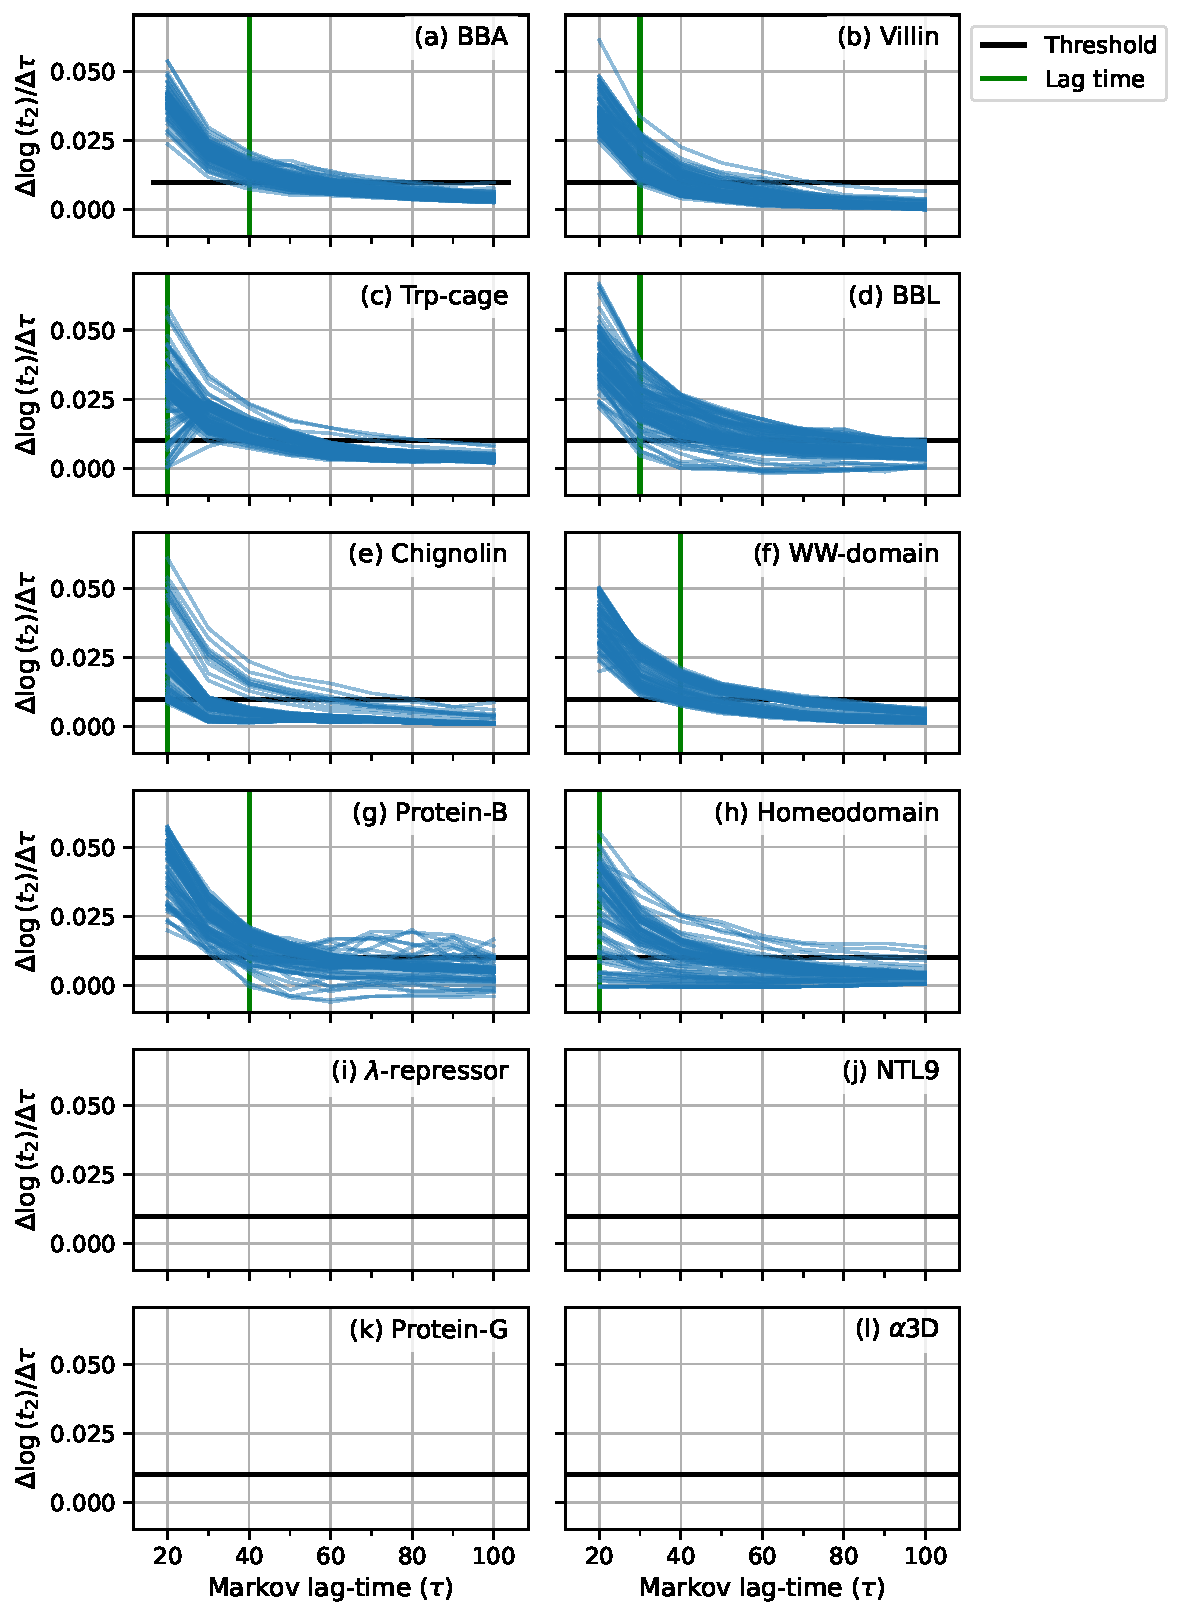
\includegraphics[height=0.8\textwidth]{figures/t_2_gradient_sharey_True_log_True_denom_delta_x.pdf}
    \caption{\textsc{Implied timescale gradient for all hyperparameter trials.} Each panel shows $\Delta t_{2}/\Delta \tau$: gradient of the dominant timescale ($t_{2}$) with respect to the Markov lag-time. The gradient was calculated for each bootstrap sample and then the median was taken. The horizontal black line is the threshold for determining the lag time. The vertical blue line is the chosen lag-time.}
    \label{fig:t2_gradient}
\end{figure}


\subsection{Hyperparameter relevance and information sharing}

\begin{figure}
    \centering
    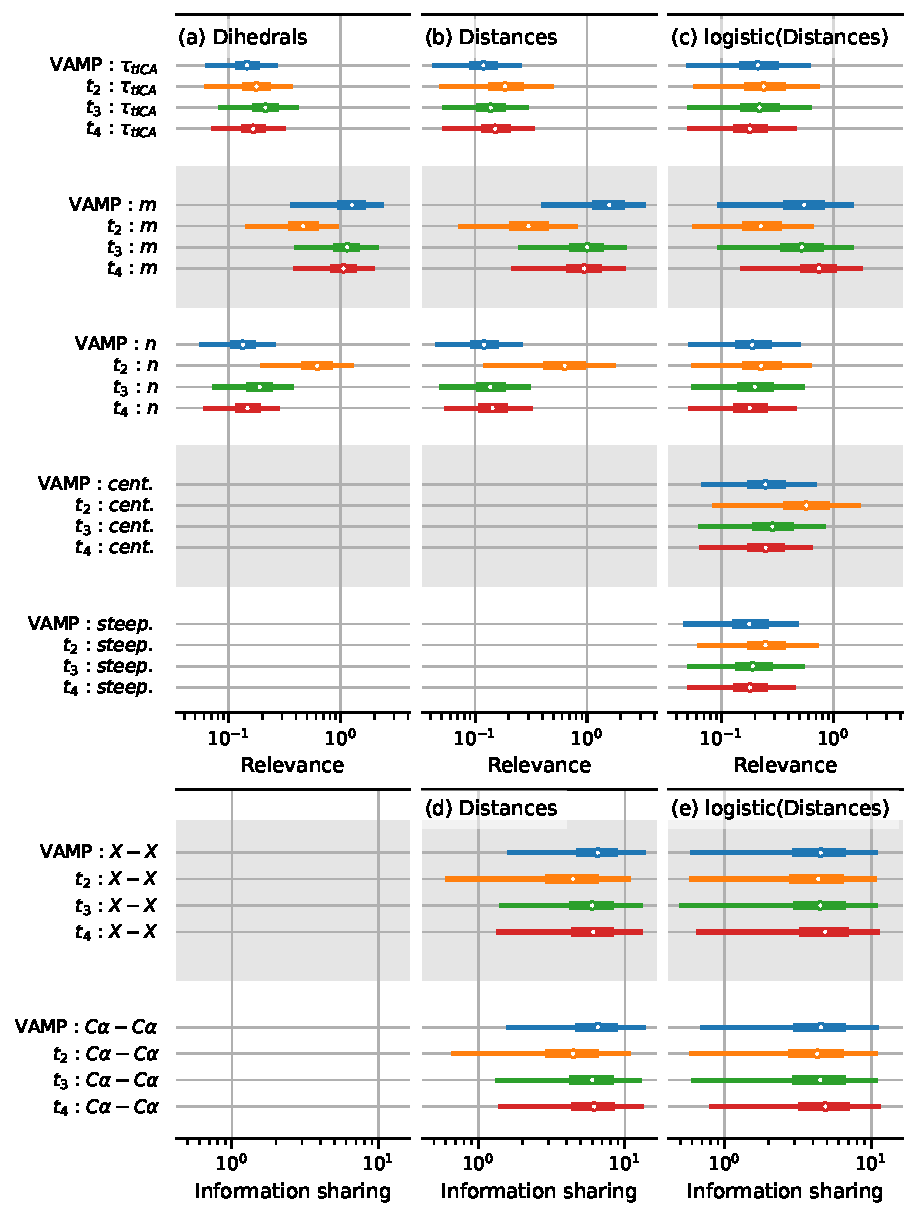
\includegraphics[height=0.8\textheight]{figures/sensitivities/1fme_sensitivity.pdf}
    \caption{\textsc{BBA hyperparameter relevance and information sharing}. Shown are the  median (white dot), \SI{50}{\percent} and \SI{95}{\percent} credible intervals (thick and thin lines respectively).  Panels (a)-(c) show the hyperparameter relevance for of each hyperparameter in determining the log of the VAMP-2 score (`VAMP' in blue) and the log of the dominant timescales ($t_{2}, t_{3}, ...$ in orange, green etc.). $\tau_{\mathrm{tICA}}$ is the TICA lag-time; $m$ is the TICA dimension, $n$ is the number of cluster centers; $cent.$ and $steep.$ are the center and steepness parameters of the logistic transform. Panels (d)-(e) show the information sharing parameters for whether the contact distances use the `closest-heavy' ($X-X$) or the `alpha-carbon' ($C_{\alpha}-C_{\alpha}$) scheme.  }
    \label{fig:1fme_sense}
\end{figure}


\begin{figure}
    \centering
    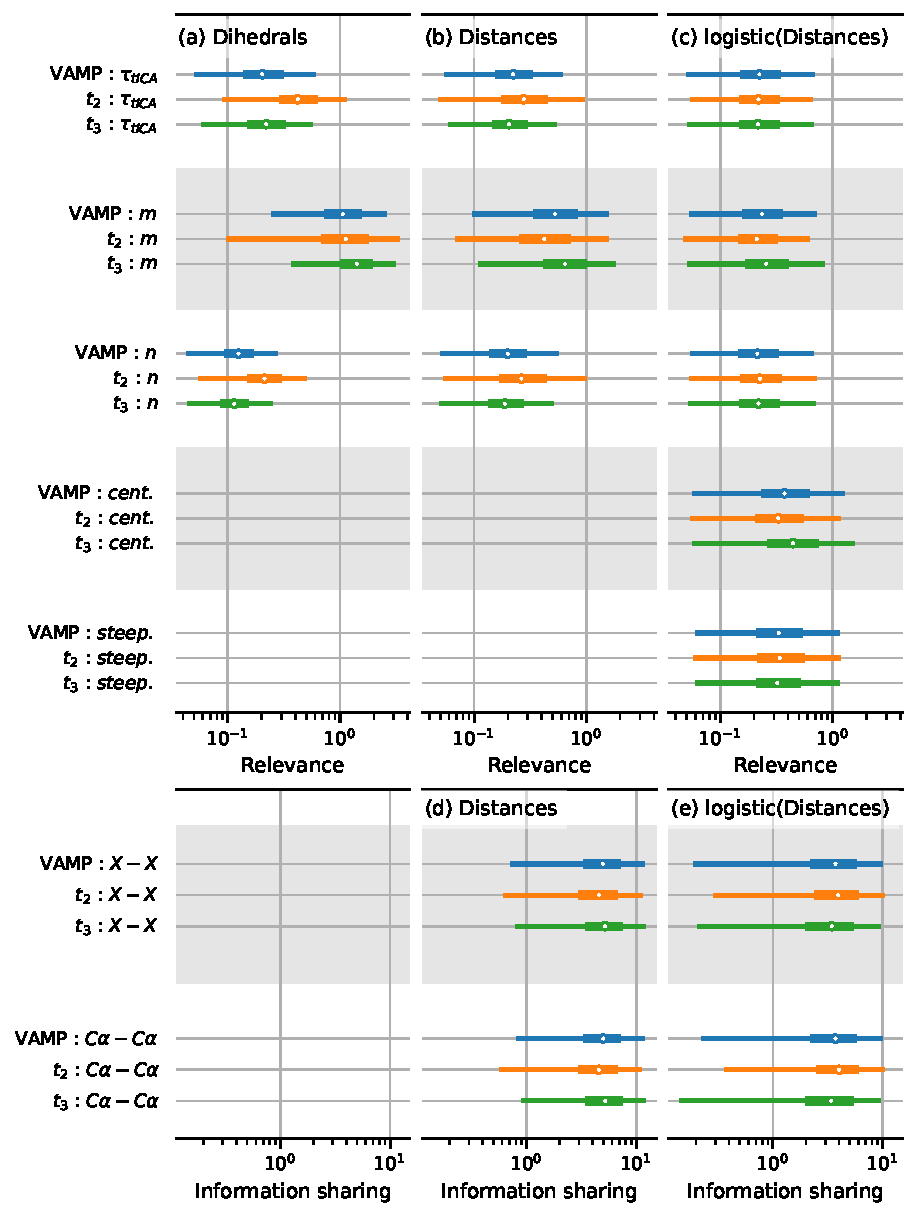
\includegraphics[height=0.8\textheight]{figures/sensitivities/2f4k_sensitivity.pdf}
    \caption{\textsc{Villin hyperparameter relevance and information sharing}. Shown are the  median (white dot), \SI{50}{\percent} and \SI{95}{\percent} credible intervals (thick and thin lines respectively).  Panels (a)-(c) show the hyperparameter relevance for of each hyperparameter in determining the log of the VAMP-2 score (`VAMP' in blue) and the log of the dominant timescales ($t_{2}, t_{3}, ...$ in orange, green etc.). $\tau_{\mathrm{tICA}}$ is the TICA lag-time; $m$ is the TICA dimension, $n$ is the number of cluster centers; $cent.$ and $steep.$ are the center and steepness parameters of the logistic transform. Panels (d)-(e) show the information sharing parameters for whether the contact distances use the `closest-heavy' ($X-X$) or the `alpha-carbon' ($C_{\alpha}-C_{\alpha}$) scheme.  }
    \label{fig:2f4k_sense}
\end{figure}

\begin{figure}
    \centering
    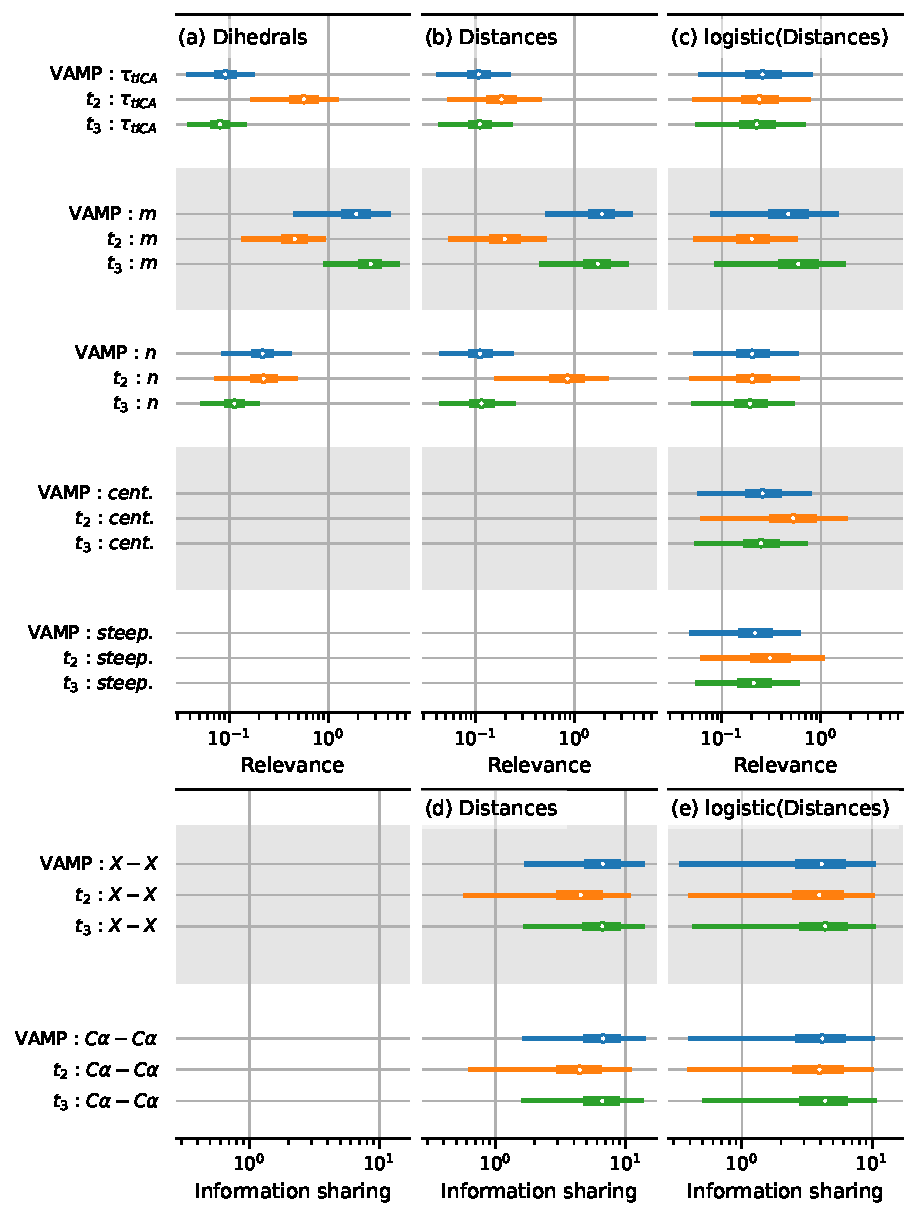
\includegraphics[height=0.8\textheight]{figures/sensitivities/2jof_sensitivity.pdf}
    \caption{\textsc{Trp-cage hyperparameter relevance and information sharing}. Shown are the  median (white dot), \SI{50}{\percent} and \SI{95}{\percent} credible intervals (thick and thin lines respectively).  Panels (a)-(c) show the hyperparameter relevance for of each hyperparameter in determining the log of the VAMP-2 score (`VAMP' in blue) and the log of the dominant timescales ($t_{2}, t_{3}, ...$ in orange, green etc.). $\tau_{\mathrm{tICA}}$ is the TICA lag-time; $m$ is the TICA dimension, $n$ is the number of cluster centers; $cent.$ and $steep.$ are the center and steepness parameters of the logistic transform. Panels (d)-(e) show the information sharing parameters for whether the contact distances use the `closest-heavy' ($X-X$) or the `alpha-carbon' ($C_{\alpha}-C_{\alpha}$) scheme.  }
    \label{fig:2jof_sense}
\end{figure}

\begin{figure}
    \centering
    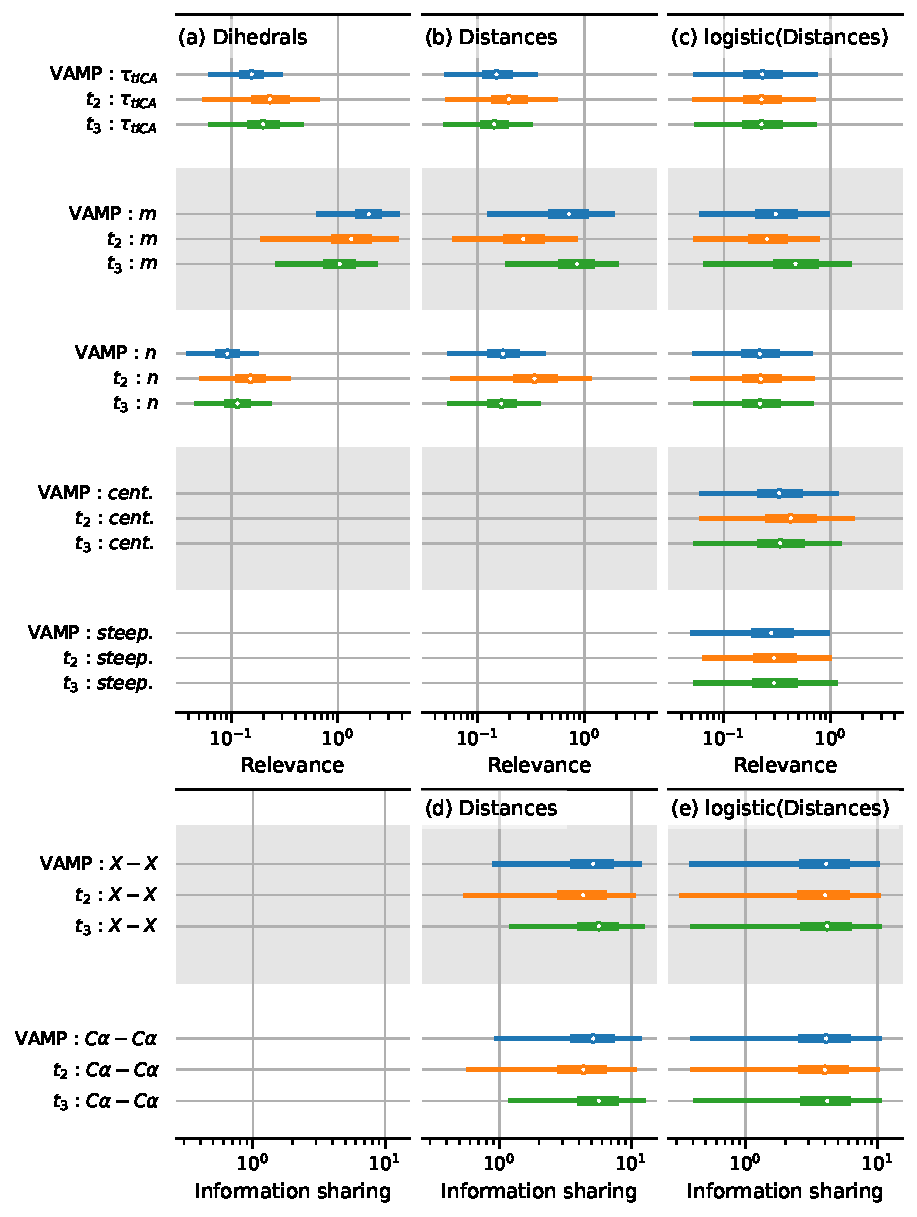
\includegraphics[height=0.8\textheight]{figures/sensitivities/2wav_sensitivity.pdf}
    \caption{\textsc{BBL hyperparameter relevance and information sharing}. Shown are the  median (white dot), \SI{50}{\percent} and \SI{95}{\percent} credible intervals (thick and thin lines respectively).  Panels (a)-(c) show the hyperparameter relevance for of each hyperparameter in determining the log of the VAMP-2 score (`VAMP' in blue) and the log of the dominant timescales ($t_{2}, t_{3}, ...$ in orange, green etc.). $\tau_{\mathrm{tICA}}$ is the TICA lag-time; $m$ is the TICA dimension, $n$ is the number of cluster centers; $cent.$ and $steep.$ are the center and steepness parameters of the logistic transform. Panels (d)-(e) show the information sharing parameters for whether the contact distances use the `closest-heavy' ($X-X$) or the `alpha-carbon' ($C_{\alpha}-C_{\alpha}$) scheme.  }
    \label{fig:2wav_sense}
\end{figure}

\begin{figure}
    \centering
    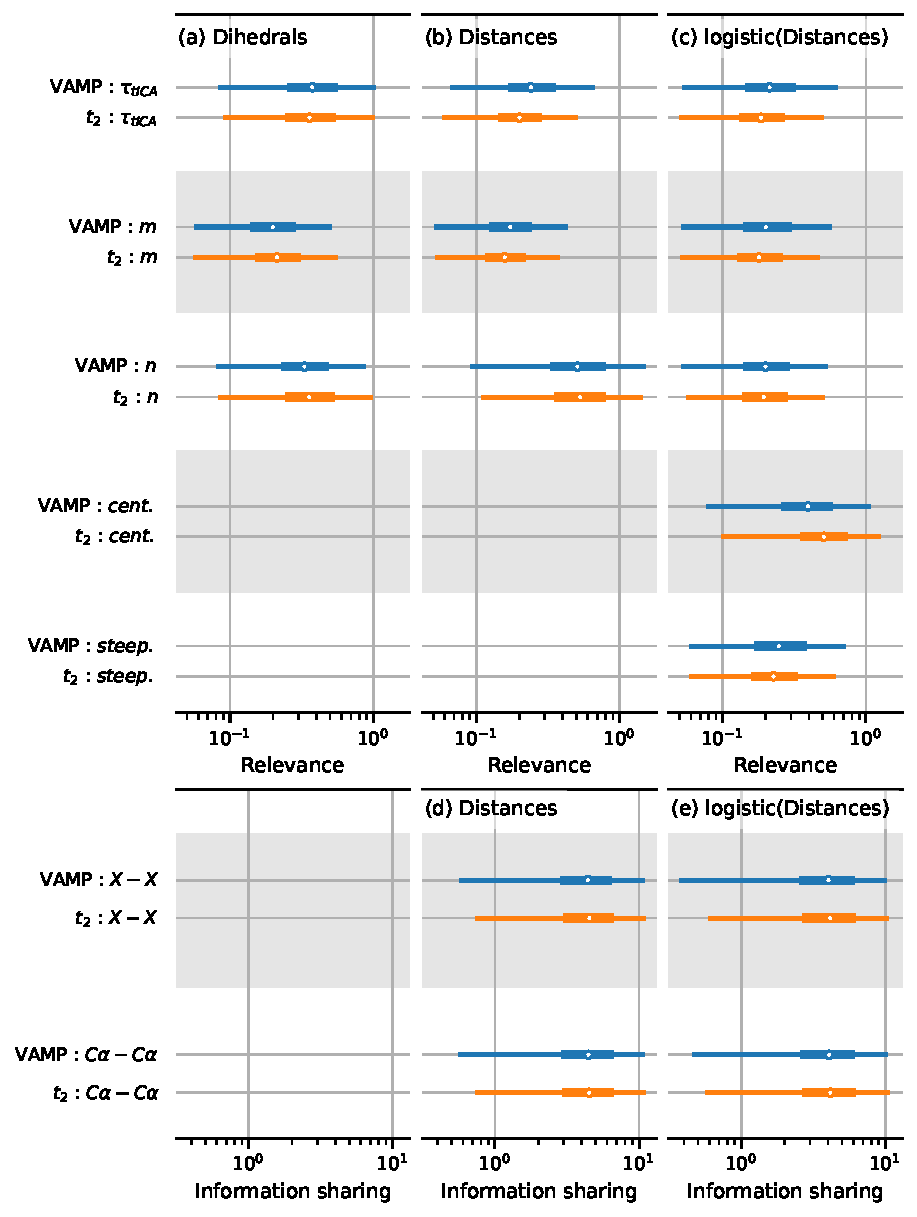
\includegraphics[height=0.8\textheight]{figures/sensitivities/cln025_sensitivity.pdf}
    \caption{\textsc{Chignolin hyperparameter relevance and information sharing}. Shown are the  median (white dot), \SI{50}{\percent} and \SI{95}{\percent} credible intervals (thick and thin lines respectively).  Panels (a)-(c) show the hyperparameter relevance for of each hyperparameter in determining the log of the VAMP-2 score (`VAMP' in blue) and the log of the dominant timescales ($t_{2}, t_{3}, ...$ in orange, green etc.). $\tau_{\mathrm{tICA}}$ is the TICA lag-time; $m$ is the TICA dimension, $n$ is the number of cluster centers; $cent.$ and $steep.$ are the center and steepness parameters of the logistic transform. Panels (d)-(e) show the information sharing parameters for whether the contact distances use the `closest-heavy' ($X-X$) or the `alpha-carbon' ($C_{\alpha}-C_{\alpha}$) scheme.  }
    \label{fig:cln025_sense}
\end{figure}

\begin{figure}
    \centering
    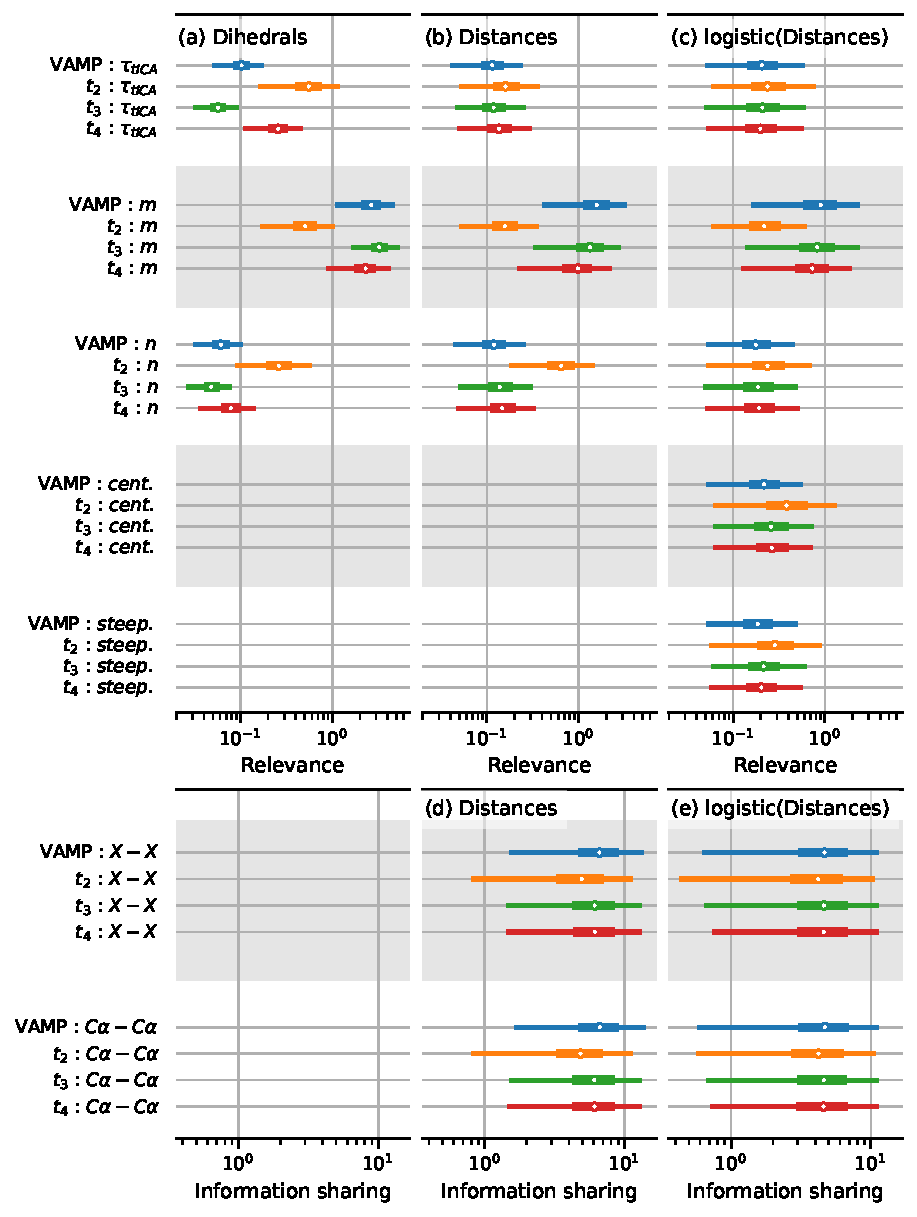
\includegraphics[height=0.8\textheight]{figures/sensitivities/gtt_sensitivity.pdf}
    \caption{\textsc{WW-domain hyperparameter relevance and information sharing}. Shown are the  median (white dot), \SI{50}{\percent} and \SI{95}{\percent} credible intervals (thick and thin lines respectively).  Panels (a)-(c) show the hyperparameter relevance for of each hyperparameter in determining the log of the VAMP-2 score (`VAMP' in blue) and the log of the dominant timescales ($t_{2}, t_{3}, ...$ in orange, green etc.). $\tau_{\mathrm{tICA}}$ is the TICA lag-time; $m$ is the TICA dimension, $n$ is the number of cluster centers; $cent.$ and $steep.$ are the center and steepness parameters of the logistic transform. Panels (d)-(e) show the information sharing parameters for whether the contact distances use the `closest-heavy' ($X-X$) or the `alpha-carbon' ($C_{\alpha}-C_{\alpha}$) scheme.  }
    \label{fig:gtt_sense}
\end{figure}

\begin{figure}
    \centering
    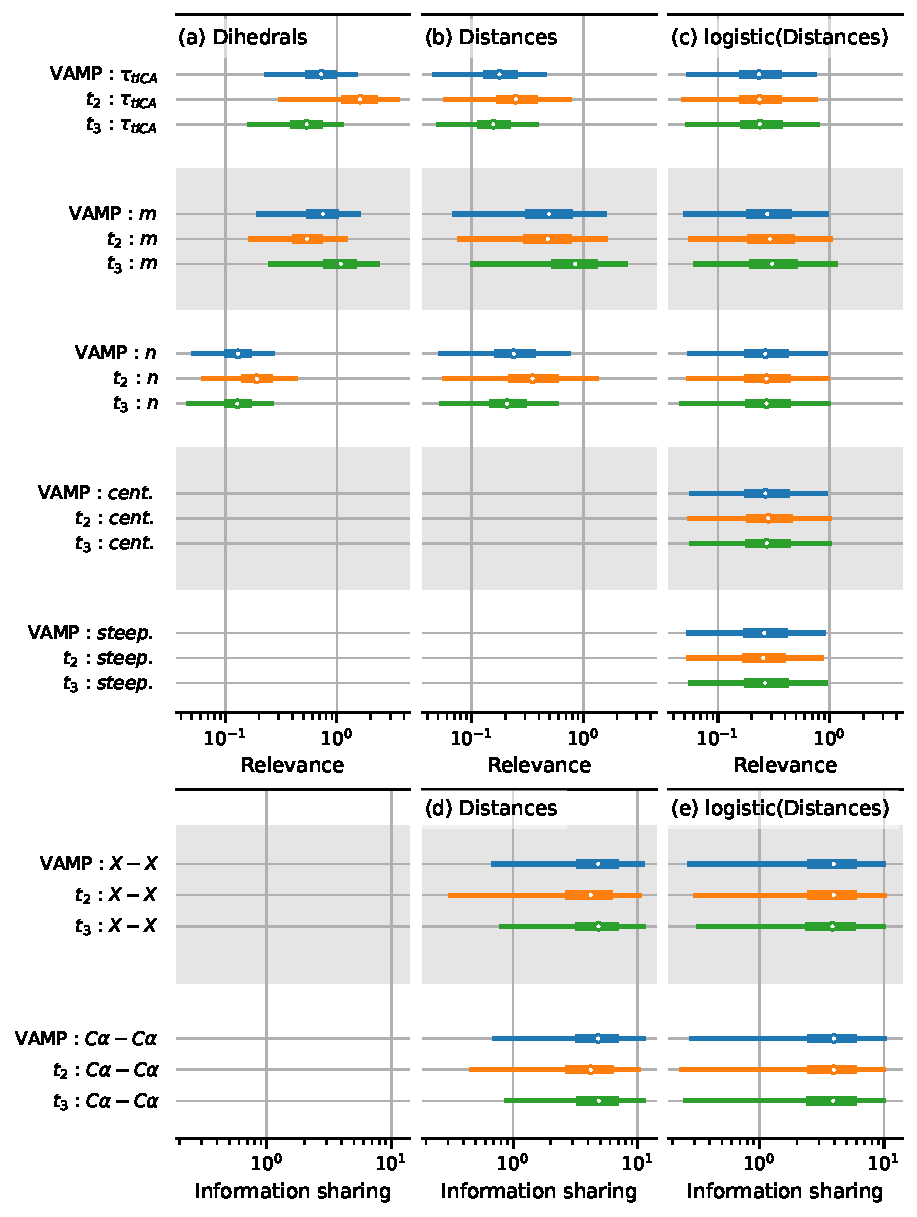
\includegraphics[height=0.8\textheight]{figures/sensitivities/prb_sensitivity.pdf}
    \caption{\textsc{Protein-B hyperparameter relevance and information sharing}. Shown are the  median (white dot), \SI{50}{\percent} and \SI{95}{\percent} credible intervals (thick and thin lines respectively).  Panels (a)-(c) show the hyperparameter relevance for of each hyperparameter in determining the log of the VAMP-2 score (`VAMP' in blue) and the log of the dominant timescales ($t_{2}, t_{3}, ...$ in orange, green etc.). $\tau_{\mathrm{tICA}}$ is the TICA lag-time; $m$ is the TICA dimension, $n$ is the number of cluster centers; $cent.$ and $steep.$ are the center and steepness parameters of the logistic transform. Panels (d)-(e) show the information sharing parameters for whether the contact distances use the `closest-heavy' ($X-X$) or the `alpha-carbon' ($C_{\alpha}-C_{\alpha}$) scheme.  }
    \label{fig:prb_sense}
\end{figure}

\begin{figure}
    \centering
    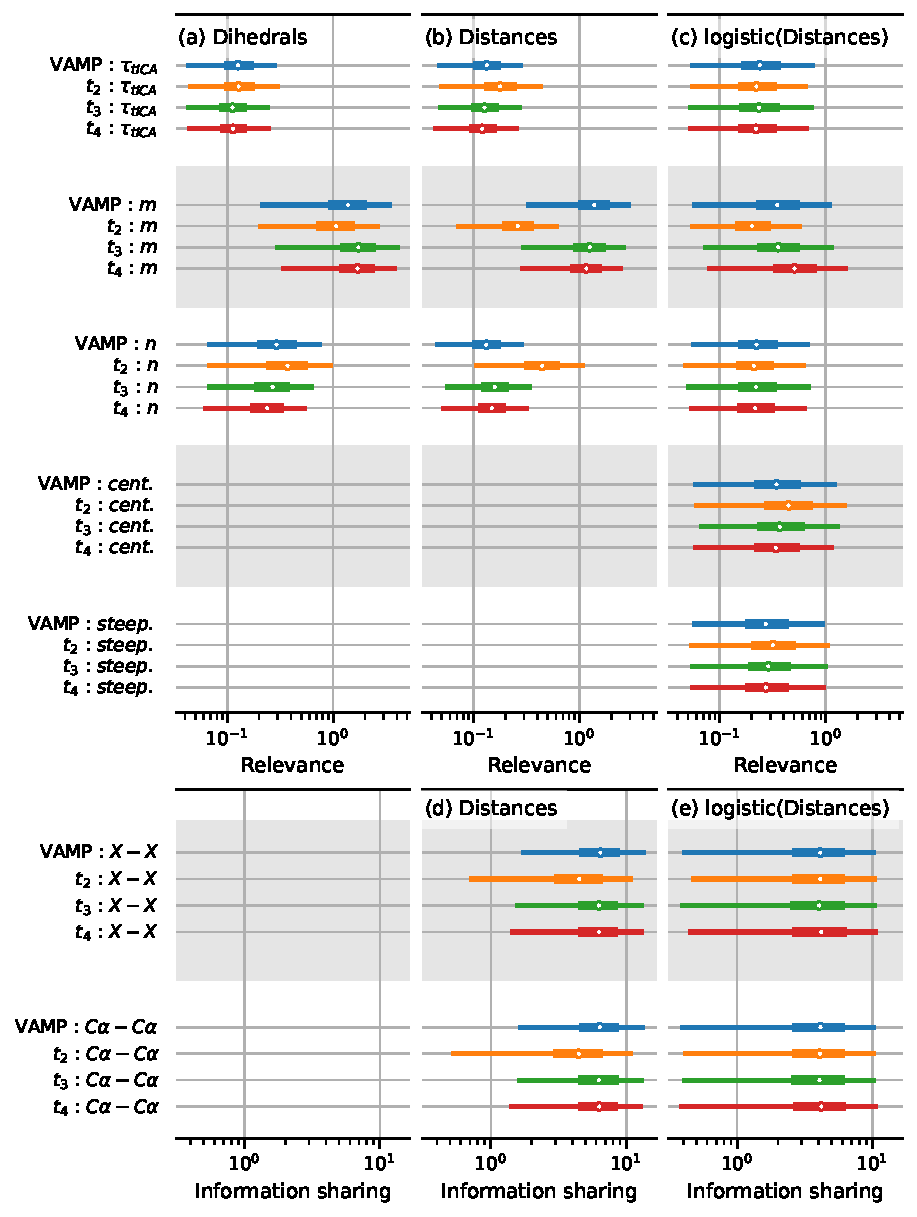
\includegraphics[height=0.8\textheight]{figures/sensitivities/uvf_sensitivity.pdf}
    \caption{\textsc{Homeodomain hyperparameter relevance and information sharing}. Shown are the  median (white dot), \SI{50}{\percent} and \SI{95}{\percent} credible intervals (thick and thin lines respectively).  Panels (a)-(c) show the hyperparameter relevance for of each hyperparameter in determining the log of the VAMP-2 score (`VAMP' in blue) and the log of the dominant timescales ($t_{2}, t_{3}, ...$ in orange, green etc.). $\tau_{\mathrm{tICA}}$ is the TICA lag-time; $m$ is the TICA dimension, $n$ is the number of cluster centers; $cent.$ and $steep.$ are the center and steepness parameters of the logistic transform. Panels (d)-(e) show the information sharing parameters for whether the contact distances use the `closest-heavy' ($X-X$) or the `alpha-carbon' ($C_{\alpha}-C_{\alpha}$) scheme.  }
    \label{fig:uvf_sense}
\end{figure}


\end{document}


